\documentclass{article}

\usepackage[margin=1.2cm, top=1cm, bottom=1.8cm]{geometry}
\pagestyle{plain}
\linespread{1.4}

\usepackage{fontspec}
\usepackage{unicode-math}
\usepackage[main=greek, english]{babel}

\setmainfont{CMU Serif}
\setsansfont{CMU Sans Serif}
\setmonofont{CMU Typewriter Text}
\setmathfont{Latin Modern Math}

\usepackage{amsmath, enumitem}
\usepackage{dirtytalk, caption, subcaption, array, graphicx}
\usepackage{titlesec}
\usepackage{soul}
\usepackage[unicode]{hyperref}
\usepackage{verbatim}

\usepackage{pdfpages}

\usepackage{tikz}
\usetikzlibrary{arrows.meta, positioning}

\hypersetup{
    hidelinks,
    bookmarksopen=true,
    bookmarksnumbered=true,
    pdftitle={Συστήματα Αναμονής - 4η Εργαστηριακή Άσκηση},
    pdfauthor={Πέππας Μιχαήλ-Αθανάσιος}
}

\newcolumntype{P}[1]{>{\centering\arraybackslash}p{#1}}
\titleformat*{\subsubsection}{\large\bfseries}

\begin{document}

\begin{center}
    {
    \Large
    {
    \textbf{ΕΘΝΙΚΟ ΜΕΤΣΟΒΙΟ ΠΟΛΥΤΕΧΝΕΙΟ\\
    ΣΧΟΛΗ ΗΛΕΚΤΡΟΛΟΓΩΝ ΜΗΧΑΝΙΚΩΝ\\
    ΚΑΙ ΜΗΧΑΝΙΚΩΝ ΥΠΟΛΟΓΙΣΤΩΝ\\}
    }

    \vspace{1.5cm}
    \rule{18cm}{0.5pt}

    Τομέας Επικοινωνιών, Ηλεκτρονικής και Συστημάτων Πληροφορικής\\
    Εργαστήριο Διαχείρισης και Βέλτιστου Σχεδιασμού Δικτύων Τηλεματικής - NETMODE\\

    \rule{18cm}{0.5pt}

    \textbf{Συστήματα Αναμονής}\\
    \textbf{$\mathbf{4^{η}}$ Εργαστηριακή Άσκηση}\\
    }
\end{center}

\vspace{0.8cm}
\begin{center}
\includegraphics[width=7cm]{EMP Logo.png}
\end{center}

\Large
{
\vspace{0.8cm}
\noindent
\textbf{Στοιχεία Φοιτητή}
\begin{itemize}
    \item Όνομα: Πέππας Μιχαήλ-Αθανάσιος
    \item Αριθμός Μητρώου: 03121026
    \item $4^{\eta}$ Εργαστηριακή Ομάδα (Δευτέρα, 12:45-14:30)
    \item Ημερομηνία Διεξαγωγής Εργαστηρίου: 30.03.2026
    \item Ημερομηνία Παράδοσης Αναφοράς: 06.04.2026
\end{itemize}
}

\newpage
\tableofcontents

\newpage
\section{Σχεδιασμός τηλεφωνικού κέντρου}

\subsection{Μοντελοποίηση του συστήματος}

Στο πρώτο μέρος της άσκησης εξετάζουμε ένα εταιρικό τηλεφωνικό κέντρο \foreignlanguage{english}{IP PBX}, το οποίο χρησιμοποιείται από $200$ εργαζομένους για εξωτερικές και εσωτερικές κλήσεις, καθώς και για \foreignlanguage{english}{voicemail}. Το σύστημα διαθέτει $50$ εξόδους (\foreignlanguage{english}{trunks / outgoing links}) και θεωρούμε ότι, όταν όλες οι έξοδοι είναι κατειλημμένες, οι νέες κλήσεις δεν απορρίπτονται αλλά τοποθετούνται σε ουρά αναμονής απείρου μήκους.

Σύμφωνα με τη θεωρία των συστημάτων αναμονής, οι κλήσεις αποτελούν τους πελάτες του συστήματος, ενώ τα trunks αποτελούν τους εξυπηρετητές. Εφόσον στην εκφώνηση δηλώνεται ρητά ότι μια κλήση που δεν μπορεί να εξυπηρετηθεί άμεσα εισέρχεται σε ουρά και δεν χάνεται, το κατάλληλο μοντέλο δεν είναι το \foreignlanguage{english}{blocking} μοντέλο Erlang B, αλλά ένα μοντέλο ουράς αναμονής τύπου Erlang C, δηλαδή ένα σύστημα πολλών εξυπηρετητών με άπειρη χωρητικότητα ουράς. Η παρατήρηση αυτή είναι ουσιαστική, γιατί καθορίζει από την αρχή αν θα μελετήσουμε πιθανότητα απόρριψης ή πιθανότητα αναμονής.

Ο συνολικός ρυθμός αφίξεων υπολογίζεται από τη δραστηριότητα των εργαζομένων. Κάθε εργαζόμενος πραγματοποιεί κατά μέσο όρο $2$ κλήσεις ανά ώρα, άρα:
\[
\lambda = 200 \cdot 2 = 400 \text{ κλήσεις/ώρα}.
\]

Η μέση διάρκεια κάθε κλήσης είναι $3$ λεπτά, δηλαδή:
\[
h = 3 \text{ min} = \frac{3}{60} = 0.05 \text{ ώρες}.
\]

Επομένως, ο ρυθμός εξυπηρέτησης κάθε trunk είναι:
\[
\mu = \frac{1}{h} = \frac{1}{0.05} = 20 \text{ κλήσεις/ώρα}.
\]

Τέλος, ο αριθμός των εξυπηρετητών είναι:
\[
c = 50.
\]

Τα παραπάνω μεγέθη αποτελούν τη βασική αριθμητική περιγραφή του συστήματος και θα χρησιμοποιηθούν στη συνέχεια για να εκτιμήσουμε αν το τηλεφωνικό κέντρο είναι ορθά διαστασιολογημένο ή όχι.

\subsection{Ερώτημα 1: Τύπος Kendall και διάγραμμα ρυθμών μετάβασης}

Ο τύπος Kendall του συγκεκριμένου τηλεφωνικού κέντρου είναι:
\[
\mathrm{M/M/50/\infty/FCFS}.
\]

Συχνά, για συντομία, το ίδιο σύστημα γράφεται και ως:
\[
\mathrm{M/M/50}.
\]

Η ερμηνεία του παραπάνω συμβολισμού είναι η εξής:
\begin{itemize}
    \item το πρώτο $\mathrm{M}$ δηλώνει ότι οι αφίξεις ακολουθούν διαδικασία Poisson,
    \item το δεύτερο $\mathrm{M}$ δηλώνει ότι οι χρόνοι εξυπηρέτησης είναι εκθετικά κατανεμημένοι,
    \item ο αριθμός $50$ δηλώνει ότι υπάρχουν $50$ παράλληλοι εξυπηρετητές,
    \item το $\infty$ δηλώνει άπειρη χωρητικότητα συστήματος, άρα δεν υπάρχει απόρριψη λόγω πλήρους ουράς,
    \item το \foreignlanguage{english}{FCFS} δηλώνει ότι οι κλήσεις εξυπηρετούνται με σειρά άφιξης.
\end{itemize}

Αν ορίσουμε ως κατάσταση του συστήματος το πλήθος $n$ των κλήσεων που βρίσκονται συνολικά στο σύστημα (σε εξυπηρέτηση ή σε αναμονή), τότε πρόκειται για διαδικασία \foreignlanguage{english}{birth-death} με:

\[
\lambda_n = \lambda = 400, \qquad n \geq 0,
\]
δηλαδή ο ρυθμός αφίξεων είναι σταθερός σε κάθε κατάσταση, και

\[
\mu_n =
\begin{cases}
n\mu, & 1 \leq n \leq 50, \\
50\mu, & n \geq 51,
\end{cases}
\]
διότι μέχρι τις $50$ ταυτόχρονες κλήσεις κάθε νέα κλήση καταλαμβάνει ένα επιπλέον trunk, ενώ για περισσότερες από $50$ κλήσεις όλα τα trunks είναι ήδη απασχολημένα και οι επιπλέον κλήσεις απλώς περιμένουν στην ουρά.

Στο Σχήμα~\ref{fig:pbx_birth_death} φαίνεται το αντίστοιχο διάγραμμα ρυθμών μετάβασης, προσαρμοσμένο στα δεδομένα της άσκησης.

\begin{figure}[h!]
\centering
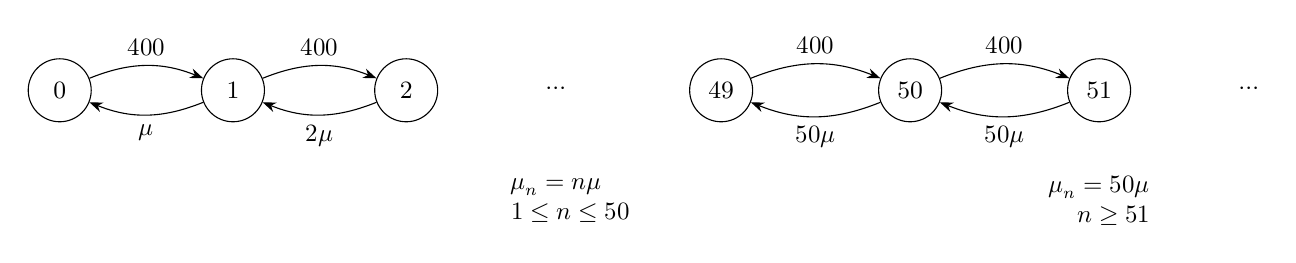
\begin{tikzpicture}[
    >=Stealth,
    state/.style={circle, draw, minimum size=8mm, inner sep=0pt},
    every node/.style={font=\small}
]
\node[state] (s0) at (0,0) {0};
\node[state] (s1) at (2.2,0) {1};
\node[state] (s2) at (4.4,0) {2};
\node (d1) at (6.3,0) {$\cdots$};
\node[state] (s49) at (8.4,0) {49};
\node[state] (s50) at (10.8,0) {50};
\node[state] (s51) at (13.2,0) {51};
\node (d2) at (15.1,0) {$\cdots$};

\draw[->, bend left=22] (s0) to node[above] {$400$} (s1);
\draw[->, bend left=22] (s1) to node[below] {$\mu$} (s0);

\draw[->, bend left=22] (s1) to node[above] {$400$} (s2);
\draw[->, bend left=22] (s2) to node[below] {$2\mu$} (s1);

\draw[->, bend left=22] (s49) to node[above] {$400$} (s50);
\draw[->, bend left=22] (s50) to node[below] {$50\mu$} (s49);

\draw[->, bend left=22] (s50) to node[above] {$400$} (s51);
\draw[->, bend left=22] (s51) to node[below] {$50\mu$} (s50);

\node[align=center] at (6.3,-1.4) {$\mu_n = n\mu$\\ για $1 \leq n \leq 50$};
\node[align=center] at (13.2,-1.4) {$\mu_n = 50\mu$\\ για $n \geq 51$};
\end{tikzpicture}
\caption{Διάγραμμα ρυθμών μετάβασης του τηλεφωνικού κέντρου $\mathrm{M/M/50/\infty/FCFS}$.}
\label{fig:pbx_birth_death}
\end{figure}

Από το παραπάνω διάγραμμα φαίνεται ότι το σύστημα μπορεί να δεχθεί απεριόριστο πλήθος κλήσεων συνολικά, όμως μόνο οι πρώτες $50$ εξυπηρετούνται ταυτόχρονα. Οι υπόλοιπες περιμένουν στην ουρά μέχρι να ελευθερωθεί κάποιο trunk. Αυτό συμφωνεί πλήρως με τη θεωρία των $\mathrm{M/M/c}$ συστημάτων, όπου ο συνολικός ρυθμός εξυπηρέτησης αυξάνεται όσο ενεργοποιούνται περισσότεροι εξυπηρετητές, αλλά μετά το πλήθος $c$ παραμένει σταθερός.

\subsection{Ερώτημα 2: Προσφερόμενη κίνηση (\foreignlanguage{english}{offered load})}

Η προσφερόμενη κίνηση υπολογίζεται από τον γνωστό τύπο:
\[
A = \lambda h.
\]

Με αντικατάσταση των δεδομένων της άσκησης παίρνουμε:
\[
A = 400 \cdot 0.05 = 20 \text{ Erlangs}.
\]

Άρα, η προσφερόμενη κίνηση του PBX είναι:
\[
\boxed{A = 20 \text{ Erlangs}}.
\]

Η ποσότητα αυτή εκφράζει τον μέσο φόρτο που προσφέρεται στο σύστημα από το σύνολο των χρηστών. Πρακτικά, τα $20$ Erlangs σημαίνουν ότι το τηλεφωνικό κέντρο απαιτεί κατά μέσο όρο πόρους ισοδύναμους με $20$ trunks συνεχώς απασχολημένους. Άρα, αν και το σύστημα διαθέτει $50$ trunks, ο μέσος απαιτούμενος φόρτος αντιστοιχεί σε σαφώς μικρότερο αριθμό ενεργών γραμμών. Αυτό είναι μία πρώτη ένδειξη ότι το σύστημα έχει σημαντικό περιθώριο λειτουργίας.

\subsection{Ερώτημα 3: Σύγκριση με το πραγματικό φορτίο (\foreignlanguage{english}{actual load})}

Στο συγκεκριμένο σύστημα θεωρούμε άπειρη ουρά και απουσία απόρριψης κλήσεων. Επιπλέον, η διαθέσιμη ικανότητα εξυπηρέτησης είναι:
\[
c\mu = 50 \cdot 20 = 1000 \text{ κλήσεις/ώρα},
\]
ενώ ο ρυθμός αφίξεων είναι:
\[
\lambda = 400 \text{ κλήσεις/ώρα}.
\]

Άρα το σύστημα είναι σαφώς ευσταθές, αφού:
\[
\lambda < c\mu.
\]

Εφόσον δεν υπάρχει απώλεια κλήσεων και όλες οι κλήσεις τελικά εξυπηρετούνται, το πραγματικό φορτίο που μεταφέρεται από το σύστημα είναι ουσιαστικά ίσο με το προσφερόμενο φορτίο. Επομένως:
\[
\text{actual load} = \text{offered load} = 20 \text{ Erlangs}.
\]

Η βασική παρατήρηση εδώ είναι ότι το τηλεφωνικό κέντρο διαθέτει πολύ μεγαλύτερη χωρητικότητα από αυτή που απαιτεί το μέσο προσφερόμενο φορτίο. Συνεπώς, δεν αναμένουμε έντονη συμφόρηση και οι πιθανότητες αναμονής θα είναι μικρές. Με άλλα λόγια, τα $50$ trunks είναι υπεραρκετά για μέσο φορτίο $20$ Erlangs. Από θεωρητική άποψη, αυτό σημαίνει ότι το σύστημα λειτουργεί μακριά από την περιοχή κορεσμού, όπου οι ουρές και οι καθυστερήσεις αυξάνονται απότομα.

\subsection{Ερώτημα 4: Βαθμός χρησιμοποίησης των trunks}

Ο βαθμός χρησιμοποίησης των εξόδων δίνεται από τον λόγο:
\[
\rho = \frac{A}{c}.
\]

Άρα:
\[
\rho = \frac{20}{50} = 0.4.
\]

Επομένως, ο βαθμός χρησιμοποίησης των trunks είναι:
\[
\boxed{\rho = 0.4 = 40\%}.
\]

Το αποτέλεσμα αυτό σημαίνει ότι κάθε trunk είναι απασχολημένο κατά μέσο όρο το $40\%$ του χρόνου. Ισοδύναμα, μπορούμε να πούμε ότι από τα $50$ διαθέσιμα trunks είναι απασχολημένα κατά μέσο όρο τα $20$, ενώ τα υπόλοιπα $30$ παραμένουν ελεύθερα. Αυτό επιβεβαιώνει ότι το τηλεφωνικό κέντρο έχει σημαντικό περιθώριο εξυπηρέτησης και λειτουργεί σε σχετικά άνετη περιοχή φόρτου. Ένας τέτοιος βαθμός χρησιμοποίησης θεωρείται αρκετά ασφαλής, αφού αφήνει περιθώριο για διακυμάνσεις στη ζήτηση χωρίς να οδηγεί εύκολα σε ουρές μεγάλης διάρκειας.

\subsection{Συμπέρασμα πρώτου μέρους}

Συνοψίζοντας, το εταιρικό τηλεφωνικό κέντρο μοντελοποιείται ως σύστημα:
\[
\mathrm{M/M/50/\infty/FCFS},
\]
με συνολικό ρυθμό αφίξεων $400$ κλήσεις/ώρα, μέσο χρόνο εξυπηρέτησης $3$ λεπτά ανά κλήση και προσφερόμενη κίνηση $20$ Erlangs. Το πραγματικό φορτίο συμπίπτει με το προσφερόμενο, επειδή δεν υπάρχουν απώλειες κλήσεων, ενώ ο βαθμός χρησιμοποίησης των trunks είναι μόλις $40\%$. Επομένως, το σύστημα είναι ευσταθές, επαρκώς διαστασιολογημένο και δεν αναμένεται να εμφανίζει έντονα φαινόμενα συμφόρησης στο μέσο καθεστώς λειτουργίας του. Το πρώτο αυτό μέρος δείχνει ξεκάθαρα ότι, με βάση τα δεδομένα της άσκησης, η υποδομή του PBX δεν είναι οριακή αλλά μάλλον συντηρητικά σχεδιασμένη.

\newpage
\section{Erlang C τηλεφωνικό κέντρο}

\subsection{Θεωρητικό υπόβαθρο και παραδοχές}

Στο δεύτερο μέρος της άσκησης μελετάμε ένα τηλεφωνικό κέντρο τύπου Erlang C, δηλαδή ένα σύστημα αναμονής με πολλούς εξυπηρετητές, άπειρη ουρά αναμονής και λογική \foreignlanguage{english}{First Come First Served (FCFS)}. Σε αντίθεση με το Erlang B, όπου μια κλήση απορρίπτεται όταν όλοι οι πόροι είναι κατειλημμένοι, στο Erlang C η κλήση εισέρχεται σε ουρά και περιμένει μέχρι να εξυπηρετηθεί.

Οι βασικές παραδοχές του μοντέλου είναι οι εξής:
\begin{itemize}
    \item οι αφίξεις των κλήσεων ακολουθούν διαδικασία Poisson,
    \item οι χρόνοι εξυπηρέτησης είναι εκθετικά κατανεμημένοι,
    \item κάθε εξυπηρετητής εξυπηρετεί μία μόνο κλήση κάθε φορά,
    \item οι κλήσεις εξυπηρετούνται με σειρά άφιξης,
    \item δεν υπάρχει εγκατάλειψη της ουράς,
    \item η ουρά θεωρείται απείρου μήκους.
\end{itemize}

Επομένως, το κατάλληλο μοντέλο είναι ένα σύστημα $\mathrm{M/M/N}$ με άπειρη ουρά, όπου στην παρούσα άσκηση:
\[
N = 10.
\]

Η συγκεκριμένη θεωρητική επιλογή είναι κρίσιμη, γιατί τα μεγέθη που μας ενδιαφέρουν εδώ δεν είναι η απόρριψη, αλλά η πιθανότητα αναμονής, το service level και ο μέσος χρόνος απάντησης, δηλαδή δείκτες ποιότητας εξυπηρέτησης.

\subsection{Δεδομένα του προβλήματος}

Η εκφώνηση δίνει:
\begin{itemize}
    \item ρυθμό αφίξεων
    \[
    \lambda = 100 \text{ κλήσεις/ώρα},
    \]
    \item μέση διάρκεια κλήσης
    \[
    h = 3 \text{ λεπτά} = \frac{3}{60} = 0.05 \text{ ώρες},
    \]
    \item αριθμό εξυπηρετητών
    \[
    N = 10.
    \]
\end{itemize}

Άρα ο ρυθμός εξυπηρέτησης κάθε εξυπηρετητή είναι:
\[
\mu = \frac{1}{h} = \frac{1}{0.05} = 20 \text{ κλήσεις/ώρα}.
\]

Για να υπολογιστεί αριθμητικά το \foreignlanguage{english}{Service Level}, απαιτείται και μια συγκεκριμένη χρονική προθεσμία $t$. Στην παρούσα υλοποίηση θεωρήσαμε:
\[
t = 20 \text{ sec},
\]
δηλαδή το σύνηθες όριο που χρησιμοποιείται συχνά ως σημείο αναφοράς σε εφαρμογές τηλεφωνικών κέντρων.

Παρατηρούμε ήδη ότι ο κάθε agent μπορεί να εξυπηρετεί κατά μέσο όρο $20$ κλήσεις ανά ώρα, άρα το σύνολο των $10$ agents παρέχει ονομαστική εξυπηρετική ικανότητα $200$ κλήσεων ανά ώρα. Η τιμή αυτή είναι διπλάσια από τον ρυθμό αφίξεων, κάτι που προϊδεάζει ότι το σύστημα θα έχει σχετικά μικρή αναμονή.

\subsection{Μεθοδολογία υπολογισμού}

Σύμφωνα με τη θεωρία του Erlang C, το offered load υπολογίζεται ως:
\[
A = \lambda h = \frac{\lambda}{\mu}.
\]

Η πιθανότητα μηδενικών κλήσεων στο σύστημα δίνεται από:
\[
P_0 =
\left[
\sum_{k=0}^{N-1}\frac{A^k}{k!}
+
\frac{A^N}{N!}\cdot\frac{N}{N-A}
\right]^{-1}.
\]

Η πιθανότητα μια νέα κλήση να χρειαστεί να περιμένει είναι:
\[
P_w =
\frac{A^N}{N!}\cdot\frac{N}{N-A}\cdot P_0.
\]

Στον κώδικα χρησιμοποιήθηκε και η έτοιμη συνάρτηση:
\[
P_w = \texttt{erlangc}(A,N),
\]
ώστε να επιβεβαιωθεί υπολογιστικά το αποτέλεσμα.

Για το \foreignlanguage{english}{Service Level}, δηλαδή το ποσοστό των κλήσεων που απαντώνται μέσα σε χρονικό διάστημα $t$, χρησιμοποιούμε:
\[
SL(t) = 1 - P_w e^{-(N\mu-\lambda)t}.
\]

Τέλος, ο μέσος χρόνος απάντησης (\foreignlanguage{english}{Average Speed of Answer - ASA}) δίνεται από:
\[
ASA = \frac{P_w \cdot h}{N-A}.
\]

Ως βοηθητικό μέγεθος, υπολογίζουμε επίσης τον βαθμό χρησιμοποίησης:
\[
\rho = \frac{A}{N}.
\]

Η μεθοδολογία αυτή συνδέει άμεσα τη θεωρία με την πράξη: πρώτα εκτιμούμε το προσφερόμενο φορτίο, στη συνέχεια βρίσκουμε πόσο συχνά οι κλήσεις θα χρειαστεί να περιμένουν, και τέλος μεταφράζουμε αυτήν την πιθανότητα σε επιχειρησιακά μεγέθη, όπως ο χρόνος απόκρισης και το επίπεδο εξυπηρέτησης.

\subsection{Αποτελέσματα υπολογισμών}

\subsubsection{Προσφερόμενη κίνηση $A$}

Από τον ορισμό:
\[
A = \lambda h = 100 \cdot 0.05 = 5 \text{ Erlangs}.
\]

Άρα:
\[
\boxed{A = 5 \text{ Erlangs}}.
\]

Το αποτέλεσμα αυτό σημαίνει ότι το τηλεφωνικό κέντρο δέχεται μέσο φόρτο ισοδύναμο με $5$ συνεχώς απασχολημένους εξυπηρετητές. Εφόσον υπάρχουν συνολικά $10$ εξυπηρετητές, η μέση απαίτηση του συστήματος αντιστοιχεί περίπου στο μισό της διαθέσιμης εξυπηρετικής ικανότητας, κάτι που προμηνύει καλή συμπεριφορά από πλευράς καθυστερήσεων.

\subsubsection{Πιθανότητα μηδενικών κλήσεων $P_0$}

Με εφαρμογή του τύπου του Erlang C βρίσκουμε:
\[
\boxed{P_0 = 0.0067081793}.
\]

Η τιμή αυτή εκφράζει την πιθανότητα να μην υπάρχει καμία κλήση στο σύστημα, δηλαδή ούτε σε εξυπηρέτηση ούτε σε αναμονή. Είναι πολύ μικρή, κάτι που είναι αναμενόμενο σε ένα σύστημα με συνεχή ροή αφίξεων. Πρακτικά, το αποτέλεσμα δείχνει ότι το σύστημα βρίσκεται σχεδόν πάντα σε κάποια ενεργή κατάσταση, χωρίς αυτό να σημαίνει ότι είναι και υπερφορτωμένο.

\subsubsection{Πιθανότητα αναμονής $P_w$}

Από τον τύπο Erlang C, ή ισοδύναμα από τη συνάρτηση \texttt{erlangc}, υπολογίζουμε:
\[
\boxed{P_w = 0.0361053592}.
\]

Δηλαδή, μόνο περίπου το $3.61\%$ των εισερχόμενων κλήσεων θα χρειαστεί να περιμένει στην ουρά. Το αποτέλεσμα αυτό δείχνει ότι το τηλεφωνικό κέντρο είναι αρκετά άνετα διαστασιολογημένο για το συγκεκριμένο φορτίο. Από θεωρητική άποψη, η μικρή τιμή του $P_w$ είναι συμβατή με το γεγονός ότι το occupancy δεν είναι υψηλό, αφού σε συστήματα Erlang C η πιθανότητα αναμονής αυξάνεται όσο το $\rho$ πλησιάζει τη μονάδα.

\subsubsection{Service Level}

Για χρονικό όριο $t$, το \foreignlanguage{english}{Service Level} υπολογίζεται από τη σχέση:
\[
SL(t) = 1 - P_w e^{-(N\mu-\lambda)t}.
\]

Στην παρούσα άσκηση έχουν ήδη υπολογιστεί:
\[
P_w = 0.0361053592,\qquad N = 10,\qquad \mu = 20,\qquad \lambda = 100.
\]

Άρα, με αντικατάσταση προκύπτει:
\[
SL(t) = 1 - 0.0361053592 \, e^{-(10\cdot 20 - 100)t}.
\]

Επομένως:
\[
SL(t) = 1 - 0.0361053592 \, e^{-100t}.
\]

Από την εκτέλεση του προγράμματος προκύπτει:
\[
\boxed{SL(20\text{ sec}) = 0.9792844267}.
\]

Σε ποσοστό:
\[
\boxed{SL(20\text{ sec}) = 97.9284426676\%}.
\]

Αυτό σημαίνει ότι περίπου το $97.93\%$ των κλήσεων απαντάται μέσα σε $20$ δευτερόλεπτα. Επομένως, το σύστημα επιτυγχάνει πολύ υψηλό επίπεδο εξυπηρέτησης. Το αποτέλεσμα είναι ιδιαίτερα καλό, αφού υπερβαίνει κατά πολύ τους συνήθεις επιχειρησιακούς στόχους, όπως για παράδειγμα το γνωστό $80/20$, δηλαδή το $80\%$ των κλήσεων να απαντάται μέσα σε $20$ δευτερόλεπτα.

\subsubsection{Χρόνος απάντησης (ASA)}

Για τον μέσο χρόνο απάντησης παίρνουμε:
\[
\boxed{ASA = 0.0003610536 \text{ ώρες}}.
\]

Ισοδύναμα:
\[
ASA = 0.0216632155 \text{ λεπτά}
\]
ή
\[
\boxed{ASA = 1.2997929297 \text{ sec}}.
\]

Ο μέσος χρόνος αναμονής μέχρι να απαντηθεί μια κλήση είναι επομένως μόλις περίπου $1.3$ δευτερόλεπτα, τιμή ιδιαίτερα μικρή, που επιβεβαιώνει την πολύ καλή λειτουργία του συστήματος. Το μέγεθος αυτό είναι άμεσα κατανοητό από την πλευρά της εμπειρίας του χρήστη: στην πράξη, η αναμονή είναι σχεδόν ανεπαίσθητη για τη μεγάλη πλειονότητα των κλήσεων.

\subsubsection{Βοηθητικός έλεγχος: βαθμός χρησιμοποίησης}

Παρότι δεν ζητείται ρητά στην αριθμητική επίλυση του δεύτερου μέρους, ο βαθμός χρησιμοποίησης είναι χρήσιμος ως έλεγχος ορθότητας:
\[
\rho = \frac{A}{N} = \frac{5}{10} = 0.5.
\]

Άρα:
\[
\boxed{\rho = 0.5 = 50\%}.
\]

Το αποτέλεσμα αυτό σημαίνει ότι κάθε εξυπηρετητής είναι κατά μέσο όρο απασχολημένος το μισό του χρόνου. Επομένως, υπάρχει επαρκές περιθώριο ώστε το σύστημα να απορροφά τις τυχαίες διακυμάνσεις των αφίξεων χωρίς να δημιουργεί σημαντική αναμονή. Το γεγονός ότι το occupancy είναι μέτριο και όχι οριακό εξηγεί γιατί και οι υπόλοιποι δείκτες ποιότητας, όπως το $P_w$, το $ASA$ και το $SL$, παίρνουν τόσο καλές τιμές.

\subsection{Έξοδος του προγράμματος σε Octave}

Παρακάτω παρατίθεται αυτούσια η έξοδος του προγράμματος από το Octave:

\begin{verbatim}
================ Erlang C - Lab 4 ================
lambda                  = 100.0000000000 calls/hour
h                       = 3.0000000000 minutes/call
mu                      = 20.0000000000 calls/server/hour
m                       = 10 servers
t                       = 20.0000000000 seconds
---------------------------------------------------
(a) Offered load A      = 5.0000000000 Erlangs
(b) P0                  = 0.0067081793
(c) Pw (erlangc)        = 0.0361053592
    Pw (closed-form)    = 0.0361053592
    abs difference      = 6.9388939039e-18
(d) Service Level SL(t) = 0.9792844267
                        = 97.9284426676 %
(e) ASA                 = 0.0003610536 hours
                        = 0.0216632155 minutes
                        = 1.2997929297 seconds
Extra: rho = A / m      = 0.5000000000
                        = 50.0000000000 %
===================================================
\end{verbatim}

Η ταύτιση του $P_w$ που υπολογίστηκε από την έτοιμη συνάρτηση \texttt{erlangc} με το $P_w$ που προέκυψε από τον κλειστό τύπο αποτελεί και έναν επιπλέον έλεγχο ορθότητας της υλοποίησης. Η πολύ μικρή αριθμητική διαφορά οφείλεται αποκλειστικά στη μηχανική ακρίβεια των υπολογισμών κινητής υποδιαστολής.

\subsection{Σχολιασμός αποτελεσμάτων}

Τα αποτελέσματα δείχνουν ότι το τηλεφωνικό κέντρο λειτουργεί σε ιδιαίτερα καλή περιοχή φόρτου. Το offered load είναι μόλις $5$ Erlangs, ενώ οι διαθέσιμοι εξυπηρετητές είναι $10$, γεγονός που αντιστοιχεί σε βαθμό χρησιμοποίησης $50\%$. Άρα, το σύστημα δεν λειτουργεί κοντά στα όρια κορεσμού του.

Η πιθανότητα αναμονής είναι μόνο $3.61\%$, δηλαδή η μεγάλη πλειονότητα των κλήσεων εξυπηρετείται αμέσως. Αυτό αποτυπώνεται και στο πολύ υψηλό \foreignlanguage{english}{Service Level}, που φτάνει περίπου το $97.93\%$ για χρονικό όριο $20$ δευτερολέπτων. Παράλληλα, ο μέσος χρόνος απάντησης είναι περίπου $1.3$ δευτερόλεπτα, οπότε η εμπειρία εξυπηρέτησης για τον χρήστη αναμένεται να είναι πολύ καλή.

Από θεωρητική σκοπιά, η εικόνα αυτή είναι απολύτως συνεπής με το μοντέλο $\mathrm{M/M/N}$: όταν ο λόγος $\rho = A/N$ παραμένει αρκετά κάτω από τη μονάδα, το σύστημα είναι ευσταθές και η ουρά παραμένει μικρή τις περισσότερες χρονικές στιγμές. Έτσι, το μικρό occupancy εξηγεί φυσικά και το μικρό $P_w$, ενώ το μικρό $P_w$ οδηγεί με τη σειρά του σε πολύ καλό service level και πολύ μικρό ASA.

Συνολικά, μπορούμε να συμπεράνουμε ότι για τα δεδομένα της άσκησης οι $10$ εξυπηρετητές επαρκούν πλήρως. Το σύστημα είναι ευσταθές, η αναμονή παραμένει περιορισμένη και η ποιότητα εξυπηρέτησης είναι υψηλή. Μάλιστα, μπορούμε να πούμε ότι η στελέχωση είναι μάλλον γενναιόδωρη για το συγκεκριμένο φορτίο, αφού η απόδοση που επιτυγχάνεται είναι αισθητά καλύτερη από τους συνήθεις στόχους λειτουργίας ενός τηλεφωνικού κέντρου.

\subsection{Συμπέρασμα δεύτερου μέρους}

Με εφαρμογή του μοντέλου Erlang C για $\lambda = 100$ κλήσεις/ώρα, μέση διάρκεια κλήσης $3$ λεπτά και $N = 10$ εξυπηρετητές, υπολογίσαμε offered load $A = 5$ Erlangs, πιθανότητα αναμονής $P_w \approx 0.0361$, πιθανότητα μηδενικών κλήσεων $P_0 \approx 0.0067$, \foreignlanguage{english}{Service Level} περίπου $97.93\%$ για όριο $20$ δευτερολέπτων και μέσο χρόνο απάντησης περίπου $1.3$ δευτερόλεπτα.

Τα αποτελέσματα αυτά επιβεβαιώνουν ότι η εξυπηρετική ικανότητα του συστήματος είναι περισσότερο από ικανοποιητική για τον συγκεκριμένο ρυθμό αφίξεων και τον δεδομένο χρόνο εξυπηρέτησης. Συνεπώς, το μοντέλο δείχνει ότι ο αριθμός των εξυπηρετητών είναι επαρκής και ότι το συγκεκριμένο τηλεφωνικό κέντρο μπορεί να προσφέρει πολύ υψηλή ποιότητα εξυπηρέτησης χωρίς σημαντικές καθυστερήσεις.

\newpage
\section{Προαιρετικό ερώτημα: Πρακτική διάσταση τηλεφωνικού κέντρου με στόχο Service Level}

Στην παρούσα άσκηση ο αριθμός των εξυπηρετητών δίνεται εκ των προτέρων και στη συνέχεια αξιολογούμε την απόδοση του συστήματος. Στην πράξη όμως, όπως φαίνεται και στο παράδειγμα του \foreignlanguage{english}{Erlang C calculator} που προτείνεται στην εκφώνηση, η διαδικασία σχεδιασμού ακολουθεί συνήθως την αντίστροφη πορεία: δεν θεωρούμε γνωστό τον αριθμό των agents, αλλά τον υπολογίζουμε με βάση έναν επιθυμητό στόχο ποιότητας εξυπηρέτησης. Έτσι, το Erlang C δεν λειτουργεί μόνο ως εργαλείο ανάλυσης, αλλά και ως εργαλείο διαστασιολόγησης προσωπικού.

\subsection{Γενική ιδέα της διαδικασίας}

Η πρακτική διαδικασία στελέχωσης με Erlang C περιλαμβάνει τα παρακάτω βήματα:
\begin{enumerate}
    \item υπολογίζουμε το offered load
    \[
    A = \lambda h,
    \]
    όπου $\lambda$ είναι ο ρυθμός αφίξεων και $h$ ο μέσος χρόνος χειρισμού κλήσης,
    \item επιλέγουμε έναν στόχο \foreignlanguage{english}{Service Level}, π.χ.\ $80\%$ των κλήσεων να απαντώνται μέσα σε $20$ δευτερόλεπτα,
    \item ξεκινάμε από έναν αρχικό αριθμό agents λίγο μεγαλύτερο από το offered load και αυξάνουμε επαναληπτικά το $N$,
    \item για κάθε υποψήφιο $N$ υπολογίζουμε την πιθανότητα αναμονής $P_w$ και έπειτα το service level,
    \item επιλέγουμε τον μικρότερο αριθμό agents που ικανοποιεί τον στόχο service level,
    \item ελέγχουμε αν το occupancy είναι αποδεκτό,
    \item τέλος, διορθώνουμε τον αριθμό αυτόν με βάση το shrinkage, ώστε να προκύψει ο πραγματικός προγραμματισμένος αριθμός agents.
\end{enumerate}

Η διαδικασία αυτή δείχνει ότι στη βιομηχανική πράξη δεν αρκεί να γνωρίζουμε απλώς αν ένα σύστημα είναι ευσταθές. Χρειάζεται να εξασφαλίζουμε και συγκεκριμένο επίπεδο ποιότητας, δηλαδή οι πελάτες να εξυπηρετούνται μέσα σε αποδεκτό χρόνο.

\subsection{Worked example του προτεινόμενου calculator}

Στο παράδειγμα του άρθρου θεωρούνται:
\[
100 \text{ κλήσεις ανά } 30 \text{ λεπτά},
\]
\[
AHT = 180 \text{ sec} = 3 \text{ λεπτά},
\]
\[
\text{Service Level target} = 80\% \text{ σε } 20 \text{ sec},
\]
\[
\text{Maximum Occupancy} = 85\%,
\]
\[
\text{Shrinkage} = 30\%.
\]

Αρχικά, οι $100$ κλήσεις ανά $30$ λεπτά αντιστοιχούν σε:
\[
200 \text{ κλήσεις/ώρα}.
\]

Άρα το offered load είναι:
\[
A = 200 \cdot \frac{3}{60} = 10 \text{ Erlangs}.
\]

Το άρθρο ξεκινά από έναν αρχικό αριθμό agents ίσο με $A+1$, δηλαδή $N=11$, και στη συνέχεια αυξάνει τον αριθμό των agents μέχρι να ικανοποιηθεί ο στόχος service level. Στο συγκεκριμένο παράδειγμα παρουσιάζονται αναλυτικά τα εξής ενδιάμεσα αποτελέσματα:
\begin{itemize}
    \item για $N=12$, το service level είναι $64.0\%$,
    \item για $N=13$, το service level είναι $79.6\%$,
    \item για $N=14$, το service level είναι $88.8\%$.
\end{itemize}

Επομένως, ο μικρότερος αριθμός agents που πετυχαίνει τον στόχο $80/20$ είναι:
\[
\boxed{N_{\text{raw}} = 14}.
\]

Ο αριθμός αυτός αποκαλείται \foreignlanguage{english}{raw number of agents}, δηλαδή ο καθαρός απαιτούμενος αριθμός agents πριν ληφθούν υπόψη πρόσθετοι πρακτικοί περιορισμοί όπως το occupancy και το shrinkage. Είναι σημαντικό ότι οι $13$ agents δεν αρκούν, παρότι βρίσκονται πολύ κοντά στον στόχο, γιατί στη σχεδίαση τέτοιων συστημάτων μας ενδιαφέρει η ελάχιστη τιμή που ικανοποιεί πραγματικά το ζητούμενο επίπεδο απόδοσης.

\subsection{Έλεγχος occupancy}

Αφού βρεθεί ο ελάχιστος αριθμός agents που ικανοποιεί τον στόχο service level, το επόμενο βήμα είναι ο έλεγχος του occupancy. Το άρθρο ορίζει το occupancy ως το ποσοστό του χρόνου κατά το οποίο οι agents είναι απασχολημένοι με την εξυπηρέτηση πελατών. Για το παράδειγμα με $A=10$ Erlangs και $N=14$ agents, προκύπτει:
\[
\text{Occupancy} = \frac{A}{N}\cdot 100
= \frac{10}{14}\cdot 100
= 71.4\%.
\]

Η τιμή αυτή είναι μικρότερη από το όριο $85\%$ που είχε τεθεί ως μέγιστο αποδεκτό occupancy, άρα οι $14$ agents παραμένουν αποδεκτοί και από αυτήν την άποψη. Αν το occupancy ξεπερνούσε το όριο, θα χρειαζόταν περαιτέρω αύξηση του αριθμού agents. Η ύπαρξη αυτού του ελέγχου είναι ουσιαστική, γιατί ένα σύστημα μπορεί θεωρητικά να πετυχαίνει τον στόχο service level, αλλά να λειτουργεί πολύ κοντά στα όριά του, με αποτέλεσμα έντονη πίεση στο προσωπικό.

\subsection{Διόρθωση με shrinkage}

Το τελευταίο βήμα είναι η ενσωμάτωση του shrinkage. Όπως εξηγεί το άρθρο, το shrinkage χρησιμοποιείται ώστε να ληφθεί υπόψη το γεγονός ότι ένα μέρος του προσωπικού δεν είναι συνεχώς διαθέσιμο για παραγωγική εξυπηρέτηση λόγω αδειών, ασθενειών, εκπαίδευσης, συναντήσεων και άλλων μη παραγωγικών δραστηριοτήτων. Για shrinkage $30\%$, ο τελικός απαιτούμενος προγραμματισμένος αριθμός agents είναι:
\[
N_{\text{scheduled}}
=
\frac{N_{\text{raw}}}{1-\text{shrinkage}}
=
\frac{14}{1-0.30}
=
\frac{14}{0.70}
=
20.
\]

Άρα το τελικό συμπέρασμα του παραδείγματος είναι ότι, ενώ ο καθαρός απαιτούμενος αριθμός για να επιτευχθεί ο στόχος service level είναι $14$ agents, στην πράξη πρέπει να προγραμματιστούν:
\[
\boxed{20 \text{ agents}}.
\]

Η διαφορά αυτή είναι ιδιαίτερα σημαντική, διότι δείχνει ότι η θεωρητική στελέχωση με Erlang C πρέπει να μετατρέπεται σε ρεαλιστική στελέχωση λαμβάνοντας υπόψη πραγματικούς επιχειρησιακούς παράγοντες. Με άλλα λόγια, άλλο είναι το παραγωγικά απαιτούμενο προσωπικό και άλλο το συνολικό προσωπικό που πρέπει να είναι προγραμματισμένο στο σύστημα.

\subsection{Σχόλιο σε σχέση με την παρούσα άσκηση}

Στη δική μας άσκηση ο αριθμός των εξυπηρετητών δίνεται εξαρχής, άρα δεν χρειάστηκε να γίνει αναζήτηση του ελάχιστου $N$ που επιτυγχάνει συγκεκριμένο στόχο service level. Ωστόσο, το προαιρετικό αυτό ερώτημα είναι χρήσιμο γιατί δείχνει πώς χρησιμοποιείται το Erlang C σε πραγματικές εφαρμογές τηλεφωνικών κέντρων.

Πιο συγκεκριμένα, στην πράξη η διαδικασία δεν σταματά στον υπολογισμό του $P_w$ ή του $ASA$ για δεδομένο $N$, αλλά ακολουθεί την εξής λογική:
\begin{enumerate}
    \item υπολογίζουμε το offered load,
    \item αυξάνουμε το $N$ μέχρι να ικανοποιηθεί ο στόχος service level,
    \item ελέγχουμε το occupancy ώστε να μην υπερφορτώνονται οι agents,
    \item διορθώνουμε προς τα πάνω με shrinkage για να βρούμε το πραγματικά απαιτούμενο προσωπικό.
\end{enumerate}

Επομένως, το προτεινόμενο \foreignlanguage{english}{calculator} δεν αλλάζει τη θεωρητική βάση του μοντέλου Erlang C, αλλά δείχνει πώς η θεωρία αυτή επεκτείνεται σε ένα πιο ρεαλιστικό πρόβλημα διαστασιολόγησης προσωπικού σε τηλεφωνικό κέντρο. Το σημείο αυτό είναι και η βασική αξία του προαιρετικού ερωτήματος, αφού συνδέει τους μαθηματικούς τύπους της άσκησης με την πραγματική λειτουργία ενός call center.

\newpage
\section{Παράρτημα Υλοποίησης σε Octave}

\subsection{Κώδικας Υλοποίησης}

\includepdf[pages=-]{lab4.pdf}

\newpage
\subsection{Έξοδος Προγράμματος}

\includepdf[pages=-]{lab4_output.pdf}

\end{document}
